%(BEGIN_QUESTION)
% Copyright 2006, Tony R. Kuphaldt, released under the Creative Commons Attribution License (v 1.0)
% This means you may do almost anything with this work of mine, so long as you give me proper credit

Skriv en ligning for hver av kretsene under, som viser hvordan alle spenningene i hver krets henger sammen:

$$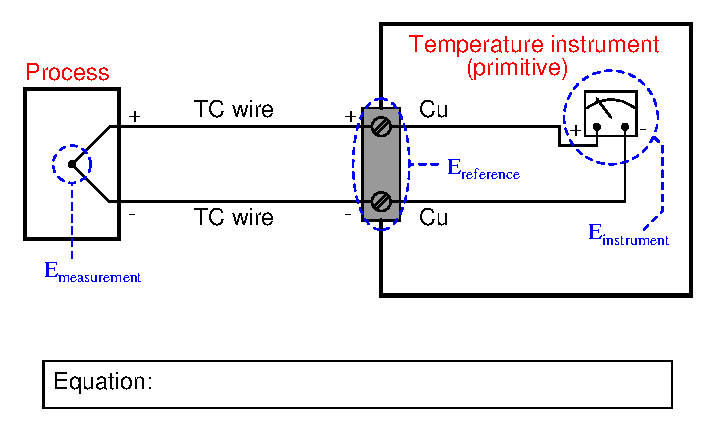
\includegraphics[width=15.5cm]{i00387x01.eps}$$

\vskip 10pt

$$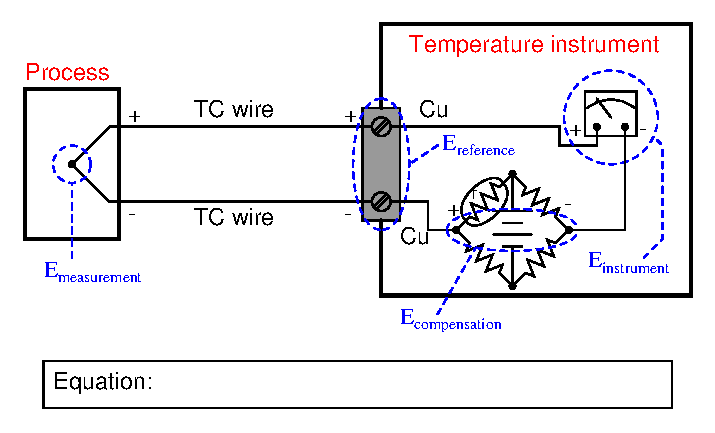
\includegraphics[width=15.5cm]{i00387x02.eps}$$

\vfil \eject

$$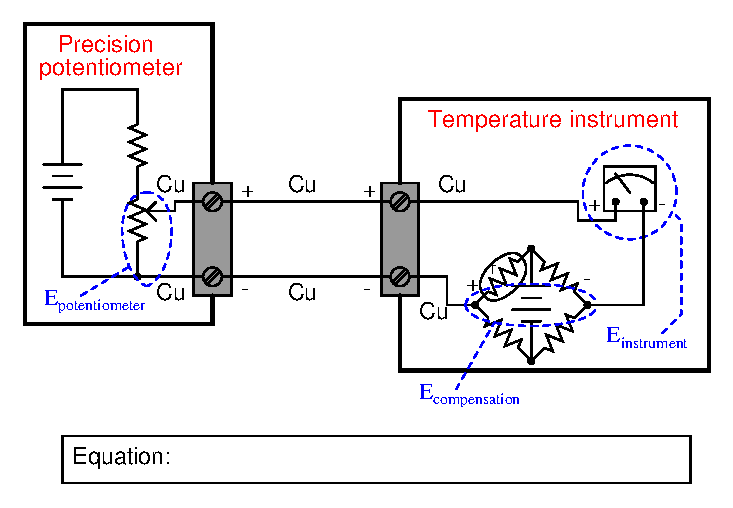
\includegraphics[width=15.5cm]{i00387x03.eps}$$

\vskip 10pt

$$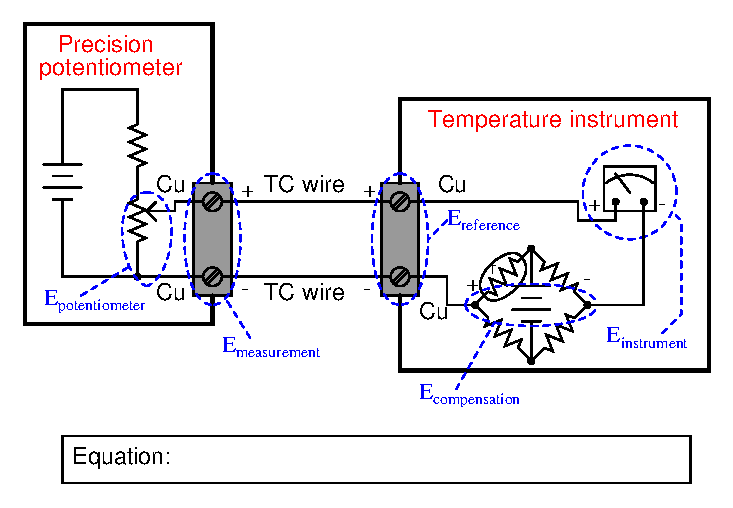
\includegraphics[width=15.5cm]{i00387x04.eps}$$

\vskip 20pt \vbox{\hrule \hbox{\strut \vrule{} {\bf Forslag til sokratisk diskusjon} \vrule} \hrule}

\begin{itemize}
\item{} Du vil se en tydelig progresjon i kompleksitet fra første til siste krets. Hvorfor tror du kretsene er satt opp i denne rekkefølgen? Hvordan kan dette hjelpe deg å sette opp ligning for realistiske kalibreringskretser senere, når du ikke har referanse tilgjengelig?
\end{itemize}

\underbar{file i00387}
%(END_QUESTION)





%(BEGIN_ANSWER)

$$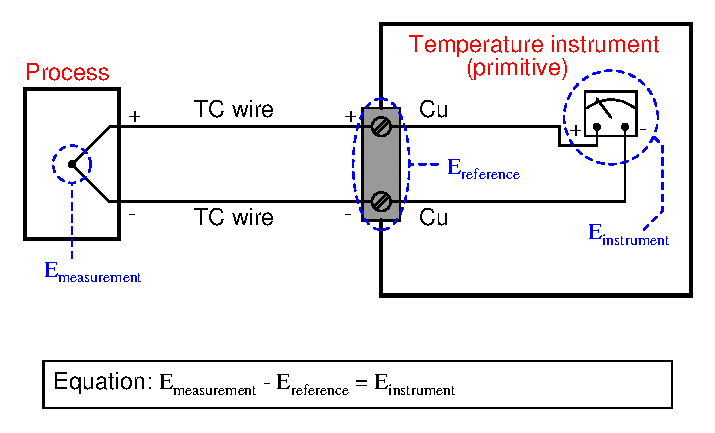
\includegraphics[width=15.5cm]{i00387x05.eps}$$

\vskip 10pt

$$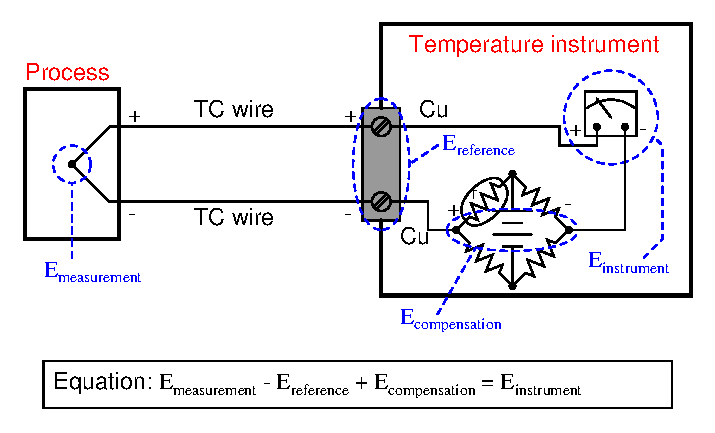
\includegraphics[width=15.5cm]{i00387x06.eps}$$

\vskip 10pt

$$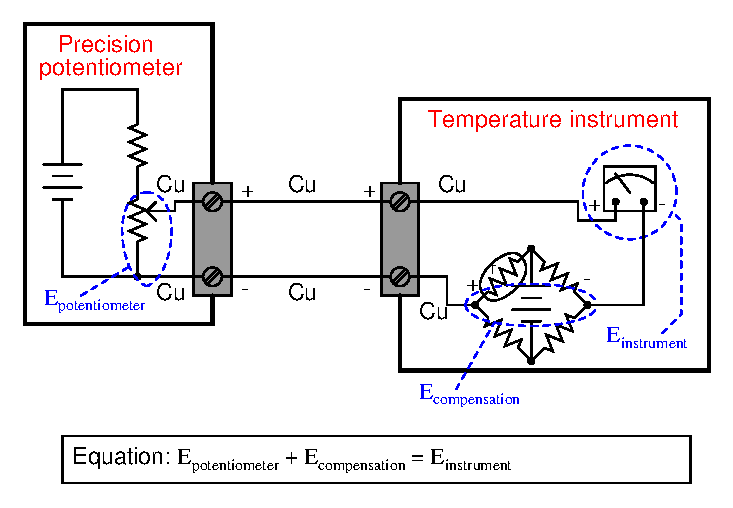
\includegraphics[width=15.5cm]{i00387x07.eps}$$

\vskip 10pt

$$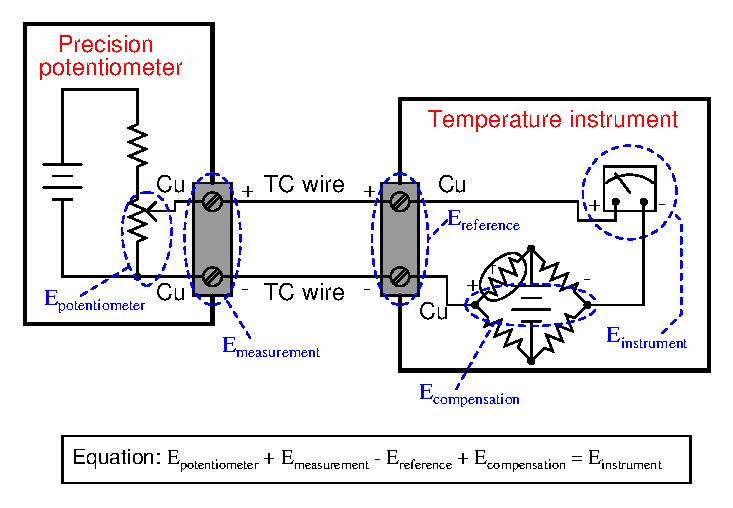
\includegraphics[width=15.5cm]{i00387x08.eps}$$

\vskip 10pt

Forenklet tommelfingerregel: Hvis du vil finne riktig potensiometerinnstilling for å generere en ønsket indikasjon på et termoelementinstrument, slå opp millivolt for ønsket temperatur og trekk fra millivolten som tilsvarer temperaturen der enten (A) kobberledninger går inn i et kompensert instrument, eller (B) termoelementledninger går inn i en intern-kobber, ukompensert kalibreringsenhet (forutsatt lik temperatur ved kalibreringsenhet og måleinstrument).

%(END_ANSWER)





%(BEGIN_NOTES)


%INDEX% Measurement, temperature: thermocouple circuit equations

%(END_NOTES)
